% LaTeX Template for short student reports.
% Citations should be in bibtex format and go in references.bib
\documentclass[a4paper, 11pt]{article}
\usepackage[top=3cm, bottom=3cm, left = 2cm, right = 2cm]{geometry} 
\geometry{a4paper} 
\usepackage[utf8]{inputenc}
\usepackage{textcomp}
\usepackage{graphicx} 
\usepackage{amsmath,amssymb}  
\usepackage{bm}  
\usepackage[pdftex,bookmarks,colorlinks,breaklinks]{hyperref}  
\usepackage{memhfixc} 
\usepackage{pdfsync}  
\usepackage{fancyhdr}
\usepackage{hyperref}
\pagestyle{fancy}
\graphicspath{ {./images/} }

\title{390R Final Writeup on the Wyze Cam V2}
\author{Ian Anderson \& Nam Nyguen\\\large \href{https://github.com/figamin/cs390r-final-wyze-cam}{Public Github Repository}} 

\date{\today}

\begin{document}
\maketitle

\section{Overview}
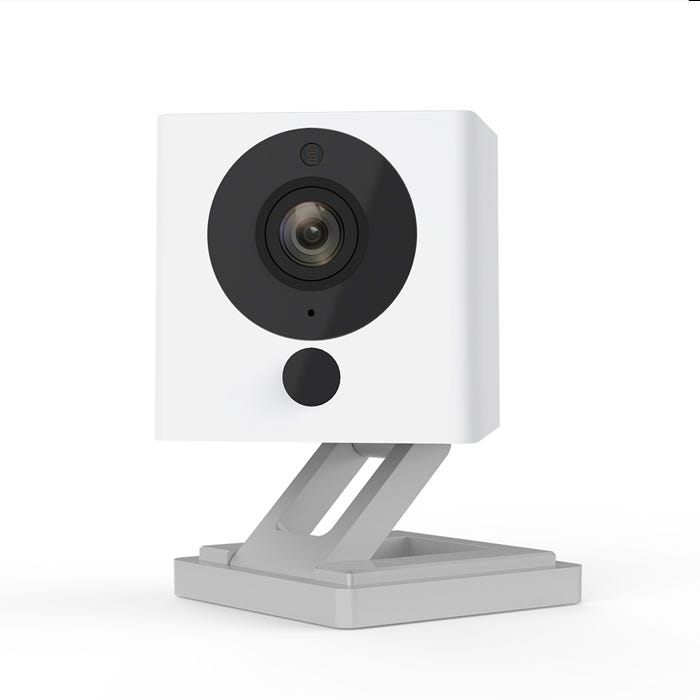
\includegraphics[scale=0.5]{wyze}\newline
The Wyze Cam V2 is a low cost security camera (MSRP \$26) developed by Wyze Labs, Inc. As with most Wyze cameras, it is largely a licenced copy of an existing Xiaomi camera, in this case being based on the Xiaomi Xiaofang 1S.\newline\newline
Some notable features of this camera include:
\begin{itemize}
    \item 1080p sensor with a 110 degree wide angle lens
    \item F2.0 aperture + 4 infrared LEDs, good for low light
    \item Speaker \& microphone for two way communication, so it can be used as an intercom
    \item Accompanying mobile app to see live video feed, capture images \& bitrate information
    \item microSD card slot for storage 
  \end{itemize}
  Our goal with this project was to see if we could find a way to exploit security vulerabilities in this camera through the process of extracting and examining it's firmware.
\section{Technical Details}
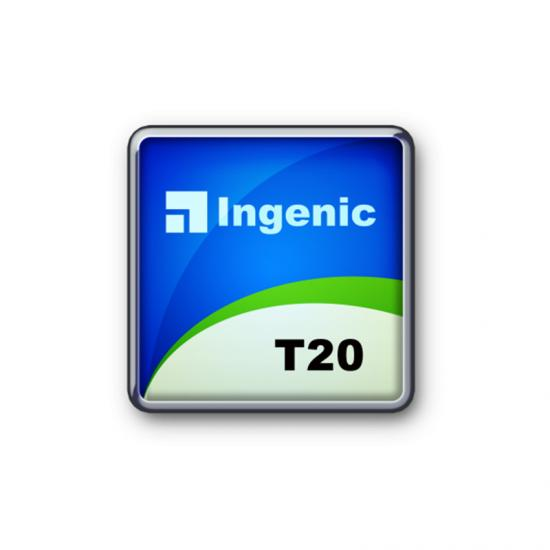
\includegraphics[scale=0.5]{ingenic}\newline
The Wyze Cam V2 is powered by the Ingenic T20 processor, an efficient SOC designed for video related IOT devices. Some of it's specs include:
\begin{itemize}
  \item "XBurst" 1GHz single core CPU based on the MIPS32 architecture
  \item 128MB of DDR2 memory
  \item Hardware H.264 encoder supporting 1080p@30fps
  \item 600mw power draw
\end{itemize}
Something that stood out on the \href{https://www.indasina.com/ingenic-t20-fhd-smart-video-processor-best-choice-for-smart-video-application_p28.html}{product info page} was "Linux BSP, GCC tool chain, Glibc", confirming that this device most likely ran Linux.
\section{Attempting to dump the firmware}
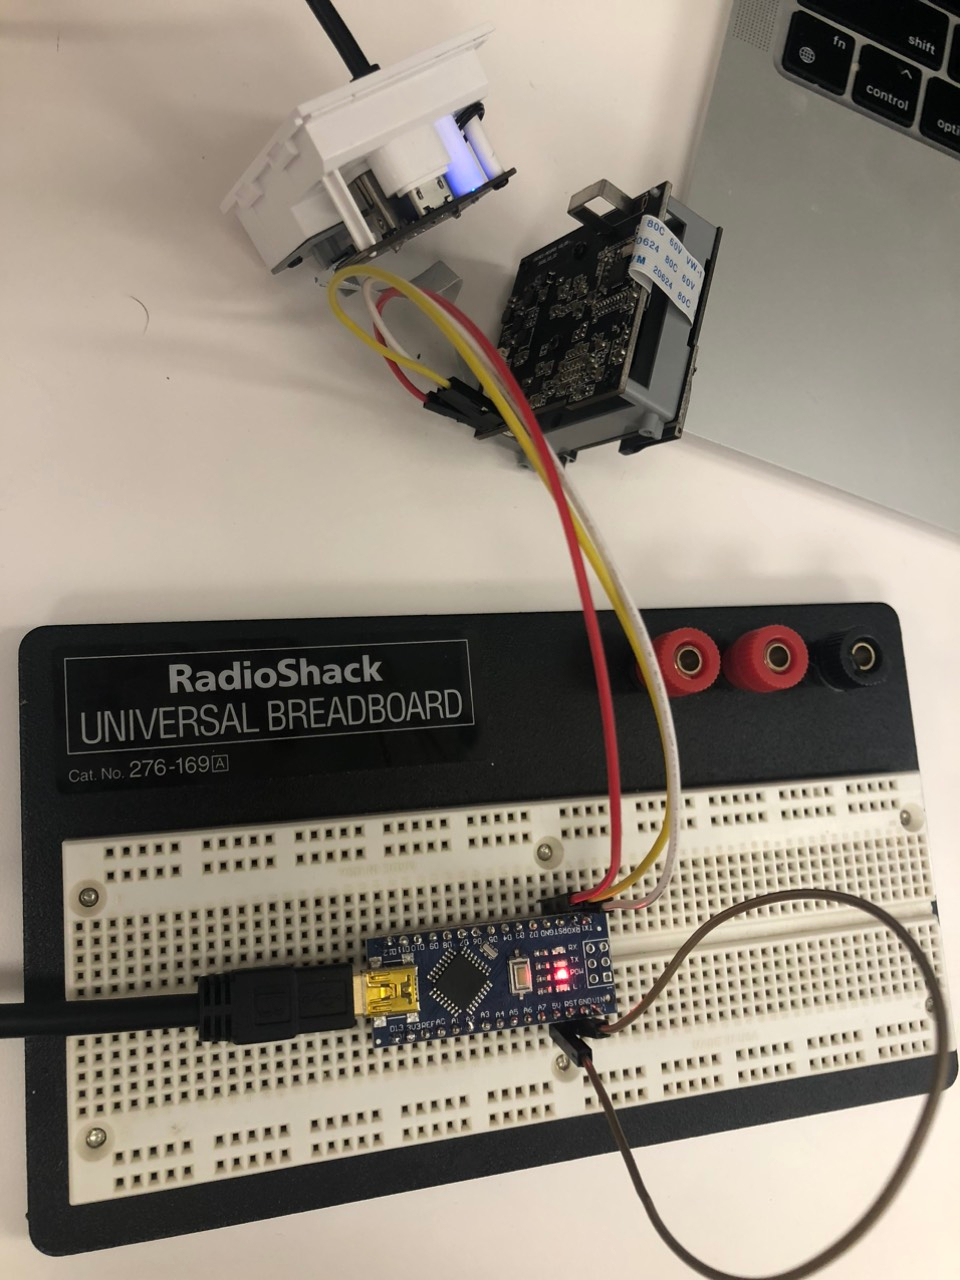
\includegraphics[scale=0.25]{image1}\newline
We obtained two cameras on eBay, and after testing one of them to make sure it was fully working, went and disassembled it until we were able to take out the main board and the attached camera board. 
To gain shell access to the Linux system, we did some research and found that \href{https://davidmac.pro/posts/2021-07-06-wyzecamv2-1-firmware/}{a hobbyist} had figured out that three pins on the edge of the main corresponded to GND, RX and TX, and used an Arduino to gain serial access to the device. Using tools in the CICS Makerspace, we were able to replicate this and get to the login, but none of the passwords we found worked for the root account, so we were not able to directly get the firmware off the device itself. However, Wyze has versions of the device's firmware avaliable for download, though these are not the standard versions. We will examine the \href{https://davidmac.pro/posts/2021-07-06-wyzecamv2-1-firmware/}{webcam firmware} found on the Wyze website. (We later found a version of the \href{https://archive.org/details/wyze_cam_rtsp_demo_bin}{RTSP firmware} that was removed from the website some time ago, but this writeup will be focued on the webcam version.)
\section{Basic examination}
To start off, one of the first things we tried was using the \verb|strings| command to see if we could find any useful data, as trying to read the binary just with \verb|cat| would just result in a bunch of garbage being outputted to the screen, and \verb|xxd| would take forever to go through with a binary of this size (11MB). To reduce the chance of simply getting a bunch of random valid characters in a row, we used the \verb|-n16| flag to only print out "words" of 16 characters or greater, which resulted in this output:
\begin{verbatim}
  Fn.record_auto_list
  AppVer=4.15.2.82
  wpa_supplicant -D nl80211 -iwlan0 -c/system/bin/wpa.conf -B &
  udhcpc -i wlan0 -p /var/run/udhcpc.pid -b &
  +m=DGEhostapd_cli
  hostapd_wpa2.conf
  '_ _ _$_$_"_"_&_&_!_!_%_%_#_#_'_'
  '? ? ?$?$?"?"?&?&?!?!?%?%?#?#?'?'
  '_ _ _$_$_"_"_&_&_!_!_%_%_#_#_'_'
  '? ? ?$?$?"?"?&?&?!?!?%?%?#?#?'?'
  mount -o nolock,rw 10.0.0.167:/home/xuxuequan/Ingenicwork/sharenfs /mnt
  restart_wlan0.sh
  az#=f02`F##f22af#3f1
  :*Fp"`D'"Fr"ad'2Fq
  az%=fP2`F%#fR2af%3fQ
  zISA_VERSION=5.6.1.32
  root:x:0:0:root:/:/bin/sh
  x:root:rJ0FHsG0ZbyZo:10933:0:99999:7:::
  webrtc_profile.ini
  wpa_supplicant.conf
  ctrl_interface=/var/run/wpa_supplicant
  model=isa.camera.isc5c1
  mac=34:CE:00:E3:FD:D7
  key=V2RX3WeYFLdWeEZc
  &PsD7p5STEDiLK4DV
  miio_client_helper_nomqtt.sh
  videobuf2-vmalloc.ko
  WH@XXH@HPDLFBDTZTPHRQRZVNAAAXBYUI^UF^A
  +8$4,<"2*9%5-=#3
  }Rlibsysutils.so
  dongle_network_add_failed.wav
  dongle_network_add_success.wav
  E6rdongle_network_start.wav
  Jdongle_sensor_delete.wav
  root:rJ0FHsG0ZbyZo:10933:0:99999:7:::
  7root:rJ0FHsG0ZbyZo:10933:0:99999:7:::
  root:rJ0FHsG0ZbyZo:10933:0:99999:7:::
  root:rJ0FHsG0ZbyZo:10933:0:99999:7:::
  =root:rJ0FHsG0ZbyZo:10933:0:99999:7:::
  iroot:rJ0FHsG0ZbyZo:10933:0:99999:7:::
  root:rJ0FHsG0ZbyZo:10933:0:99999:7:::
  Kroot:rJ0FHsG0ZbyZo:10933:0:99999:7:::
  root:rJ0FHsG0ZbyZo:10933:0:99999:7:::
  root:rJ0FHsG0ZbyZo:10933:0:99999:7:::
  K!uvc_f22.config
  root:rJ0FHsG0ZbyZo:10933:0:99999:7:::
  root:rJ0FHsG0ZbyZo:10933:0:99999:7:::
  G8uvc_jxf22.config
  uvc_jxf23.config
  [Qbnjp~iQr*V=s&:1$Lv
  @VYSGFQ]KJ^UCRNYMBFQELZ^ITRVADBFNX\JFHTRJPD\B@XL
  +8$4,<"2*9%5-=#3
  root:rJ0FHsG0ZbyZo:10933:0:99999:7:::
  croot:rJ0FHsG0ZbyZo:10933:0:99999:7:::
  libaudioProcess.so
\end{verbatim}
While a few of these were still garbage, most of this was useful information that was telling about the development of this system. For example, \verb|/home/xuxuequan/Ingenicwork/sharenfs| seems to be an NFS share used by the developers of this firmware at Ingenic. Most useful though are the shadow hashes, such as \verb|x:root:rJ0FHsG0ZbyZo:10933:0:99999:7:::|, since these can be used to potentially crack the password for the root account. To get a better idea of where these strings are, we need to explore the file system
\section{File system exploration}
To extract the file system from the firmware, we can use the tool \href{https://github.com/ReFirmLabs/binwalk}{binwalk}. Running the tool without any additional flags gives us some basic information
\begin{verbatim}
  DECIMAL       HEXADECIMAL     DESCRIPTION
  --------------------------------------------------------------------------------
  0             0x0             uImage header, header size: 64 bytes, header CRC: 0x413EFAFE,
  created: 2020-03-21 10:10:07, image size: 11075584 bytes, Data Address: 0x0, Entry Point:
  0x0, data CRC: 0xC181F3AB, OS: Linux, CPU: MIPS, image type: Firmware Image, compression 
  type: none, image name: "jz_fw"
  64            0x40            uImage header, header size: 64 bytes, header CRC: 0x7771D66A,
  created: 2020-03-20 15:44:39, image size: 1816781 bytes, Data Address: 0x80010000, Entry
  Point: 0x803E9230, data CRC: 0xBDC20C2D, OS: Linux, CPU: MIPS, image type: OS Kernel Image,
  compression type: lzma, image name: "Linux-3.10.14"
  128           0x80            LZMA compressed data, properties: 0x5D, dictionary size:
  67108864 bytes, uncompressed size: -1 bytes
  2097216       0x200040        Squashfs filesystem, little endian, version 4.0,
  compression:xz, size: 3353204 bytes, 407 inodes, blocksize: 131072 bytes,
  created:2019-05-21 17:22:45
  5570624       0x550040        Squashfs filesystem, little endian, version 4.0,
  compression:xz, size: 583802 bytes, 13 inodes, blocksize: 131072 bytes,
  created: 2020-02-23 16:07:18
  6225984       0x5F0040        JFFS2 filesystem, little endian
  8072064       0x7B2B80        JFFS2 filesystem, little endian
  8082472       0x7B5428        JFFS2 filesystem, little endian
  8162316       0x7C8C0C        Zlib compressed data, compressed
  8165504       0x7C9880        Zlib compressed data, compressed
  8168320       0x7CA380        Zlib compressed data, compressed
  8170872       0x7CAD78        JFFS2 filesystem, little endian
  ...
  11068972      0xA8E62C        JFFS2 filesystem, little endian
  11069100      0xA8E6AC        Zlib compressed data, compressed
  11070652      0xA8ECBC        JFFS2 filesystem, little endian
  11072816      0xA8F530        Zlib compressed data, compressed
\end{verbatim}
The majority of the binary is made up of the JFFS2 file system used by the Linux install (shown to be on kernel 3.10.14), with much of it being compressed. Installing \href{https://github.com/onekey-sec/jefferson/}{Jefferson}, \href{https://github.com/devttys0/sasquatch}{sasquatch} and \href{https://github.com/plougher/squashfs-tools}{squashfs-tools} allows us to run binwalk with the \verb|-e| flag and extract the root Linux filesystem.
Looking through the squashfs file system for custom files, one that immediately stuck out to me was \verb|/etc/init.d/rcS|. This is a shell script that sets up the system:
\begin{verbatim}
  #!/bin/sh

  # Set mdev
  echo /sbin/mdev > /proc/sys/kernel/hotplug
  /sbin/mdev -s && echo "mdev is ok......"
  
  # create console and null node for nfsroot
  #mknod -m 600 /dev/console c 5 1
  #mknod -m 666 /dev/null c 1 3
  
  # Set Global Environment
  export PATH=/bin:/sbin:/usr/bin:/usr/sbin
  export PATH=/system/bin:$PATH
  export LD_LIBRARY_PATH=/system/lib
  export LD_LIBRARY_PATH=/thirdlib:$LD_LIBRARY_PATH
  
  # networking
  ifconfig lo up
  #ifconfig eth0 192.168.1.80
  
  # Start telnet daemon
  telnetd &
  
  # Set the system time from the hardware clock
  #hwclock -s
  
  #set the GPIO PC13 to high, make the USB Disk can be use
  cd /sys/class/gpio
  [Note: the following sentences in brackets were originally in Chinese, I used Google Translate to be able to roughly read them]
  echo 77 > export       #[Application]GPIO
  cd gpio77
  echo out > direction   #[set to output mode]
  echo 0 > active_low    #value[It is 0, which means low level] value[It is 1, indicating high level]
  echo 1 > value         #[Setting Level (Output Mode)]
  
  # Mount driver partition
  mount -t squashfs /dev/mtdblock3 /driver
  
  # Mount system partition
  mount -t jffs2 /dev/mtdblock4 /system
  
  # Mount backup partition
  #mount -t jffs2 /dev/mtdblock5 /backupk
  
  # Mount backup partition
  #mount -t jffs2 /dev/mtdblock6 /backupd
  
  # Mount backup partition
  mount -t jffs2 /dev/mtdblock7 /backupa
  
  # Mount configs partition
  mount -t jffs2 /dev/mtdblock8 /configs
  
  # Mount params partition
  mount -t jffs2 /dev/mtdblock9 /params
  
  # Format system patition if it is invalid
  if [ ! -f /system/.system ]; then
      echo "Format system partition..."
      umount -f /system
      flash_eraseall /dev/mtd4
      mount -t jffs2 /dev/mtdblock4 /system
      cd /system
      mkdir -p bin init etc/sensor lib/firmware lib/modules
      echo "#!/bin/sh" > init/app_init.sh
      chmod 755 init/app_init.sh
      touch .system
      cd /
      echo "Done"
  fi
  
  # Run init script
  if [ -f /system/init/app_init.sh ]; then
      /system/init/app_init.sh &
  fi  
\end{verbatim}
This shows how the install is broken up into a number of different file systems. Looking at the main JFFS2 file system is far more interesting. Most of it is made up of shell scripts and custom binaries. Starting off with \verb|/init/app_init.sh|:
\begin{verbatim}
  #!/bin/sh

  cd /system
  if [ -f /system/.upgrade ]; then
      cd /backupa
      echo "init upgrading!!!!!!!!!!!!"
      ./upgrade.sh
      rm /system/.upgrade
  fi
  
  ##insmod /lib/modules/tx-isp.ko isp_clk=100000000
  ##insmod /lib/modules/sensor_imx323.ko
  ##insmod /lib/modules/sensor_jxf22.ko
  ##insmod /lib/modules/sensor_ps5230.ko
  ##insmod /lib/modules/exfat.ko
  ##insmod /lib/modules/sample_motor.ko
  ##insmod /lib/modules/audio.ko
  ##insmod /lib/modules/sinfo.ko
  ##insmod /lib/modules/8189es.ko
  
  insmod /driver/tx-isp.ko isp_clk=100000000
  ##insmod /driver/sensor_imx323.ko
  #insmod /driver/sensor_jxf23.ko
  ##insmod /driver/sensor_ps5230.ko
  insmod /driver/exfat.ko
  insmod /driver/sample_motor.ko
  insmod /system/audio.ko 
  #spk_gpio=-1 sign_mode=0
  insmod /driver/sinfo.ko
  ##insmod /driver/8189es.ko
  insmod /driver/sample_pwm_core.ko
  insmod /driver/sample_pwm_hal.ko
  #insmod /driver/rtl8189ftv.ko
  insmod /system/libcomposite.ko
  insmod /system/videobuf2-vmalloc.ko
  insmod /system/usbcamera.ko
  
  sh /system/bin/led.sh &
  /system/bin/getSensorType
  /system/ucamera &
  
  #wpa_supplicant -Dwext -i wlan0 -c /system/etc/wpa_supplicant.conf -B
  #udhcpc -i wlan0 -s /system/etc/udhcpc.script -q
  
  ifconfig eth0 up
  #udhcpc -i eth0 -s /system/etc/udhcpc.script -q
  ifconfig eth0 193.169.4.222
  route add default gw 193.169.4.1
  
  mount -t nfs -o nolock 193.169.4.2:/home_b/nfsroot/ywu/ /mnt
  # open ircut
  #cp /system/bin/setir /tmp/
  #config ip address
  
  echo 63 > /sys/class/gpio/export
  echo "out" > /sys/class/gpio/gpio63/direction
  echo 1 > /sys/class/gpio/gpio63/value
  #/system/bin/carrier-server --st=imx322
  #/system/bin/singleBoadTest
  if [ -f /system/bin/.debug ]; then
      echo "root:rJ0FHsG0ZbyZo:10933:0:99999:7:::" > /system/etc/shadow
  #    /system/bin/iCamera
  else
      echo "root:x:10933:0:99999:7:::" > /system/etc/shadow
  #    /system/bin/iCamera >/dev/null 2>&1
  fi
\end{verbatim}
Something interesting that I noticed was all the commented lines. This makes sense when you consider the fact that, with the Ingenic T20 being used in a number of security cameras, that each would have different features that would require different kernel modules. Also, it is interesting that if the \verb|.debug| file exists, then the shadow file is different.
\section{Cracking the root password}
With the shadow and passwd files, we can use \href{https://www.openwall.com/john/}{John the Ripper} to crack the root password. Since the hash used is DES, this was very easy, even when using pure brute force.
First, we combine the shadow and passwd files:\newline
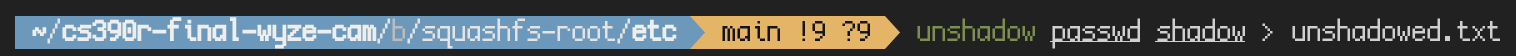
\includegraphics[scale=0.5]{screen}\newline
Then we brute force cracking the password:\newline
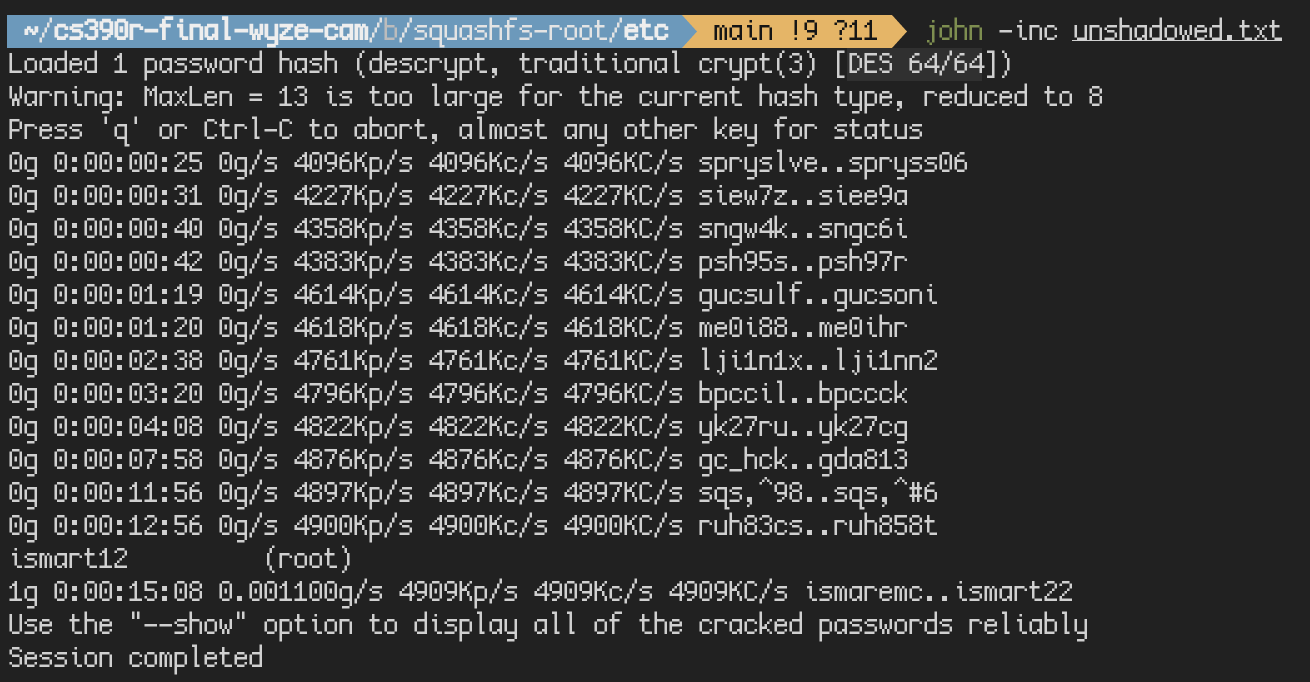
\includegraphics[scale=0.5]{screen2}\newline
So, the password ends up being \verb|ismart12|.
\section{Custom Binary analysis with Ghidra}
One more thing to look at was some of the custom binaries. Many of them are pretty simple, such as \verb|getSensorType|. Opening it with Ghidra, we can see a few interesting things.\newline
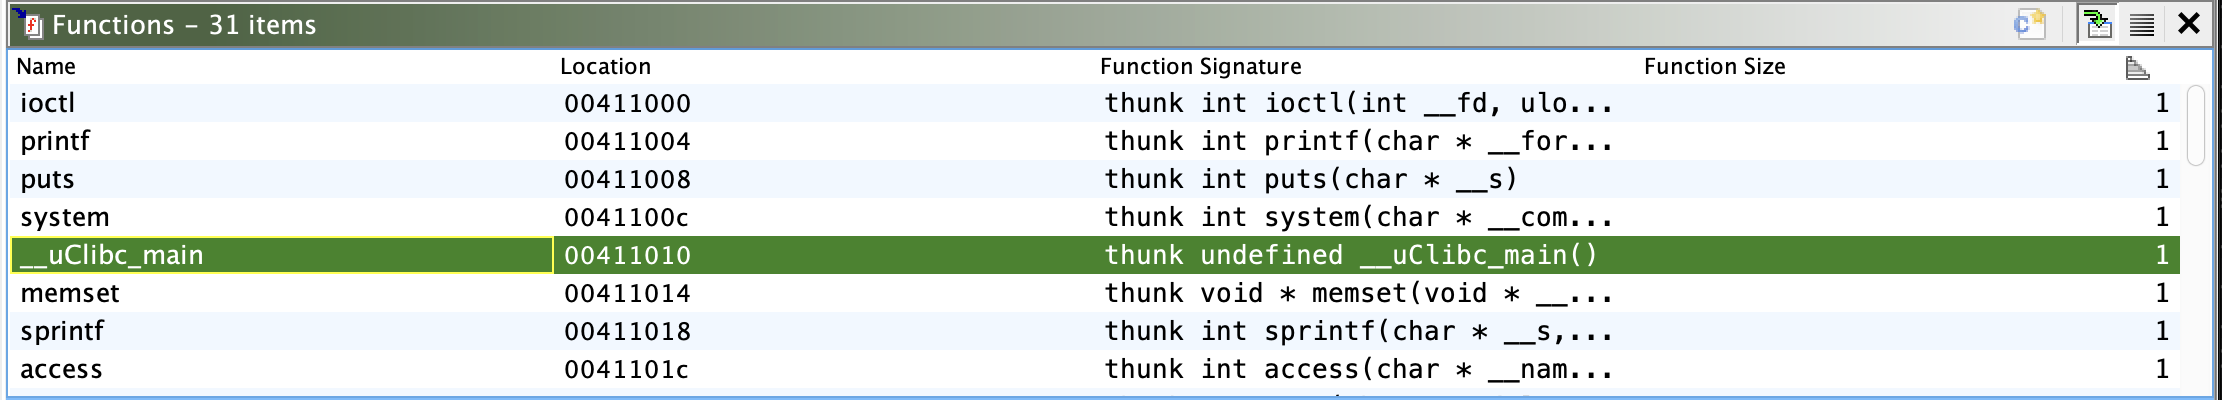
\includegraphics[scale=0.5]{uclib}\newline
First of all, all of these binaries were compiled with \href{https://www.uclibc.org/}{uClibc}, a C library meant for embedded systems such as this one.\newline
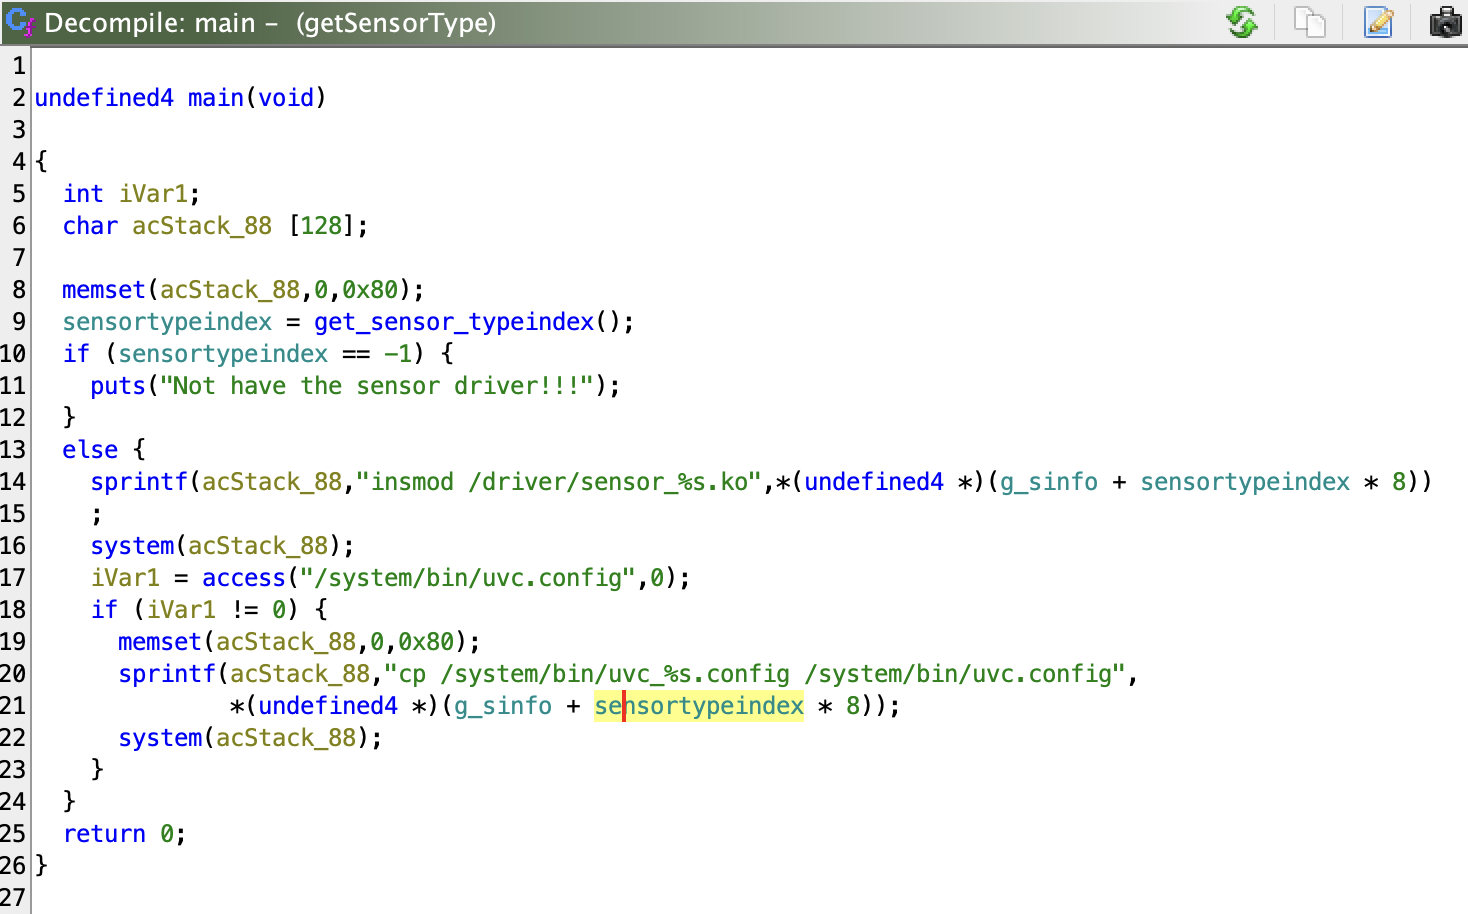
\includegraphics[scale=0.5]{main}\newline
Here is the main function of this program. As you can see, it opens a config file before trying to get the sensor type.\newline
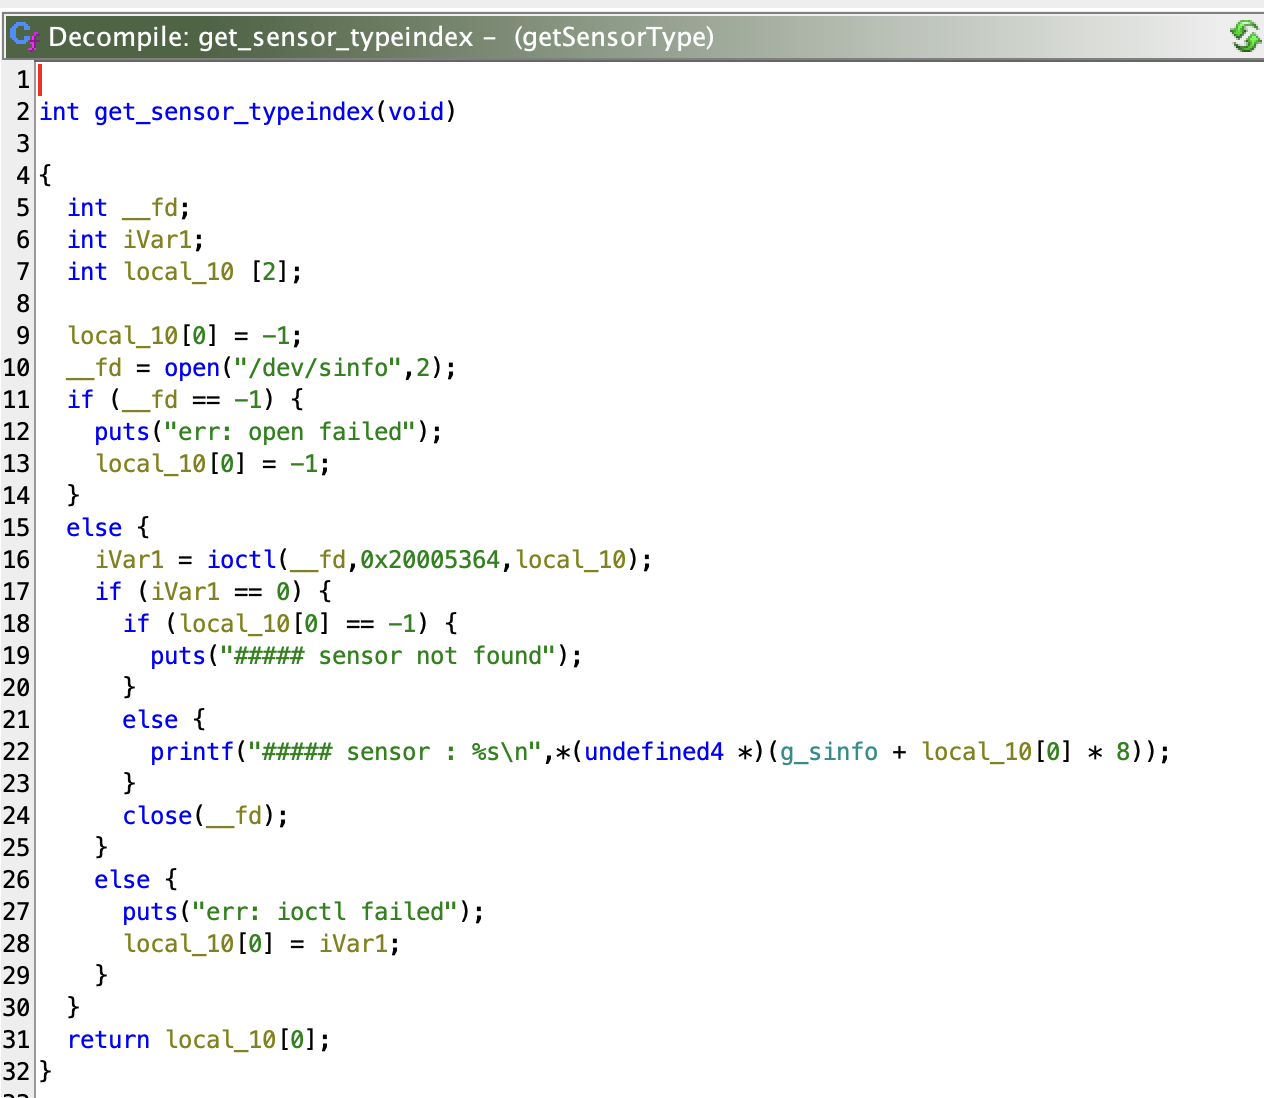
\includegraphics[scale=0.5]{sensortype}\newline
To get the sensor type, it simply opens \verb|/dev/sinfo| and checks if a certain IO device exists. There are other binaries like this in the image that do similarly simple functions
\section{Challenges}
The biggest challenge for us was getting into the file system. We initially thought this firmware would be akin to a ROM dump, and would be able to be directly analyzed in Ghidra. However, closer analysis revealed that it is more like a disk image, with its own file system that needed to be separately extracted. Additionally, getting the actual cameras took some time, as they had to be purchased by us.
\section{Further goals}
If we had more time, we would focus on analyzing all the custom binaries, looking for vulerabilities, as well as flashing this webcam firmware to one of the devices and running potential exploits on that. Since there are many custom binaries here, it is likely that at least one has potential exploits, and probably quite a few of them.
\end{document}